\chapter{Gameplay y mecánicas del juego}

% ==============================================================================

\section{Gameplay}
\subsection{Núcleo}
% \textit{En pocos párrafos, detallar la esencia del juego. Estas palabras serán las semillas a partir de las cuales el diseño del juego irá creciendo, ayudando así a que el juego tenga bastante éxito en el mercado. El contenido de esta sección es similar a la del concepto del juego pero expresado de forma más esquemática, como un listado con viñetas.}

Para que este juego tenga éxito, debemos ser capaces de encontrar un equilibrio entre la parte dinámica/caótica y la parte competitiva.

\vspace{\baselineskip}

Por una parte, la parte dinámica/caótica viene dada por:
\begin{itemize}
  \item Partidas cortas.
  \item Elementos aleatorios: El jugador elige su personaje sin conocer el mapa/objetivo ni los personajes de los otros tres jugadores.
\end{itemize}

\vspace{\baselineskip}

Por otra parte, los siguientes elementos permiten a los jugadores habilidosos controlar y contrarrestar este ``caos'', proporcionando una experiencia competitiva: 
\begin{itemize}
  \item Los jugadores pueden votar para elegir a su compañero de equipo.
  \item Una vez elegidos los equipos, se pueden mejorar algunas habilidades para adaptar al personaje a la partida actual. En la versión actual, esta característica aún no está implementada.
  \item Los chats (lobby y in-game) permiten a los jugadores coordinarse con su compañero de equipo y establecer una estrategia, incluso antes de que empiece la partida.
\end{itemize}


\subsection{Desarrollo}

A continuación se detalla cómo se produce el desarrollo de una partida:
\begin{enumerate}
   \item El jugador elige el personaje con el que va a jugar la siguiente partida. No tiene control sobre cuál va a ser el mapa de la partida ni con qué otros jugadores será emparejado en el lobby, así que debe elegir el personaje simplemente en función de lo bueno que es con él o lo mucho que le apetece jugarlo.
   \item Pulsa en el botón \emph{Search Game} y empieza la búsqueda de partida. Una vez encontrados otros tres jugadores, se le mete en el lobby con los otros jugadores.
   \item Una vez en el lobby, forma parte de una votación para crear los equipos. Puede votar para que un jugador sea su compañero de equipo y votar a otro para que sea su oponente. Esta elección teóricamente debería hacerla en función de su personaje y el de los demás. Al jugador también se le da la posibilidad de no votar. Una vez que se ha acabado el tiempo o todos los jugadores han votado, se crean los equipos teniendo en cuenta las votaciones de los usuarios. Durante esta fase, en base al chat los distintos jugadores pueden discutir sobre los distintos equipos a formar.
   \item Una vez formados los equipos, los jugadores entran en un fase donde tienen que elegir hasta dos mejoras para sus habilidades, en función de los equipos formados. Durante esta fase, se sigue pudiendo usar el chat, pero ahora solo para hablar con el compañero de equipo. Esta fase no se ha implementado aún.
   \item Tras esta fase, empieza la partida propiamente dicha. Los jugadores compiten en equipos 2v2 (formados en el lobby) intentando alcanzar un objetivo que depende del mapa de la partida. El equipo que primero alcance el objetivo es el ganador y el otro es el perdedor.
   \item Cuando la partida termina, el jugador vuelve al menú principal. En función de si ha ganado o perdido, recibe puntos de experiencia para subir de nivel y monedas que puede usar para comprar nuevos personajes con los que jugar. Además, si la partida era competitiva, gana o pierde puntos de clasificación, según haya ganado o perdido, lo que influye en su puesto en la escalera clasificatoria.
\end{enumerate}

\subsection{Progresión}
% \textit{Trazar el flujo típico con una descripción detallada de lo que tiene que hacer el jugador para ir progresando en el juego e ir cumpliendo los objetivos. Si la sección anterior era la raíz de un árbol, esta sección constituye el tronco y las ramas.}
De cara a conseguir una mayor fidelización de los jugadores, se incluyen diversos sistemas de progresión. Por una parte, hay un sistema de progresión por niveles mediante los puntos de experiencia que se consiguen al jugar partidas. Este nivel refleja la experiencia que tiene un jugador dado, en función de la cantidad de partidas jugadas.

Por otra parte, los jugadores ganan monedas al jugar partidas, más en caso de victoria que de derrota. Estas monedas se usan para desbloquear personajes con los que jugar. De esta forma, el contenido del juego se va haciendo disponible poco a poco al jugador, en vez de todo de golpe, lo que podría abrumarlo y además no le daría ninguna sensación de progresión.

Por último, al jugar partidas clasificatorias, se ganan y pierden puntos según se ganen o pierdan partidas, respectivamente, y en función de estos se establece la posición del jugador en la escalera clasificatoria. Esto proporciona una experiencia competitiva y más "seria" para aquellos jugadores más "hardcore", que se tomen en serio el juego y que quieran mejorar.

\vspace{\baselineskip}

Estos sistemas de progresión no están implementados en la versión actual del juego.

% ==============================================================================

\section{Mecánicas}
\subsection{Movimiento}
Para moverse por el escenario del mapa, los jugadores harán uso de su ratón, como suele ser el caso en la mayoría de MOBA. Al hacer click con el botón derecho en un punto del suelo, el personaje caminará (con una velocidad que dependerá de cada personaje) hacia dicha posición a través del camino más corto.

\subsection{Acciones}
Aparte del movimiento, los jugadores tendrán a su disposición 5 habilidades adicionales, que dependerán del personaje escogido. 

Para realizar el ataque básico, se deberá posicionar el cursor sobre un enemigo y pulsar el botón derecho. Si el personaje se encuentra fuera del rango del ataque básico, se moverá hasta el límite de dicho rango y entonces atacará al enemigo. 

Para el resto de habilidades, habrá que pulsar la tecla del teclado correspondiente (Q, W, E o R) y, dependiendo de la habilidad en concreto, realizar alguna acción adicional, consistente en posicionar el cursor en algún punto del mapa y presionar de nuevo (una o varias veces) la misma tecla.

\subsection{Inteligencia Artificial}
En nuestro juego, hemos usado la inteligencia artificial para dos aspectos diferentes:

\vspace{\baselineskip}

Por una parte, cuando el jugador hace click en un punto del mapa, el jugador se mueve hacia dicho punto por el camino más corto. Para encontrar el camino más corto, hemos hecho uso de los nodos \emph{Navigation} y \emph{NavigationMeshInstance}, que proporciona Godot.

Por otra parte, en el mapa \emph{Captura}, hay un hada que se desplaza por el mapa. Este hada se va moviendo de forma semialeatoria de un punto a otro del mapa, siguiendo caminos ya preestablecidos, y priorizando unos lugares sobre otros. El funcionamiento concreto se explica en el apartado de Diseño de Niveles, en el subapartado del mapa \emph{Captura}.

%  ==============================================================================

\section{Configuración}
% \textit{Detallar si el juego ofrece la posibilidad al jugador de configurar ciertos aspectos del juego. Si esto es afirmativo, explicar qué es lo que se puede modificar y su accesibilidad (por ejemplo, si el juego admite configurar la resolución de pantalla, la calidad de los gráficos, etc.).}

Por ahora, hemos implementado el menú de configuración de sonido (ver figura \ref{fig:AudioMenu}). Este menú permite al usuario configurar de forma separada el volumen maestro (que afecta a todo el sonido del juego), el volumen de la música y el volumen de los efectos de sonido. Además, se puede directamente silenciar cada uno de estos volúmenes por separado.

\begin{figure}
	\centering
	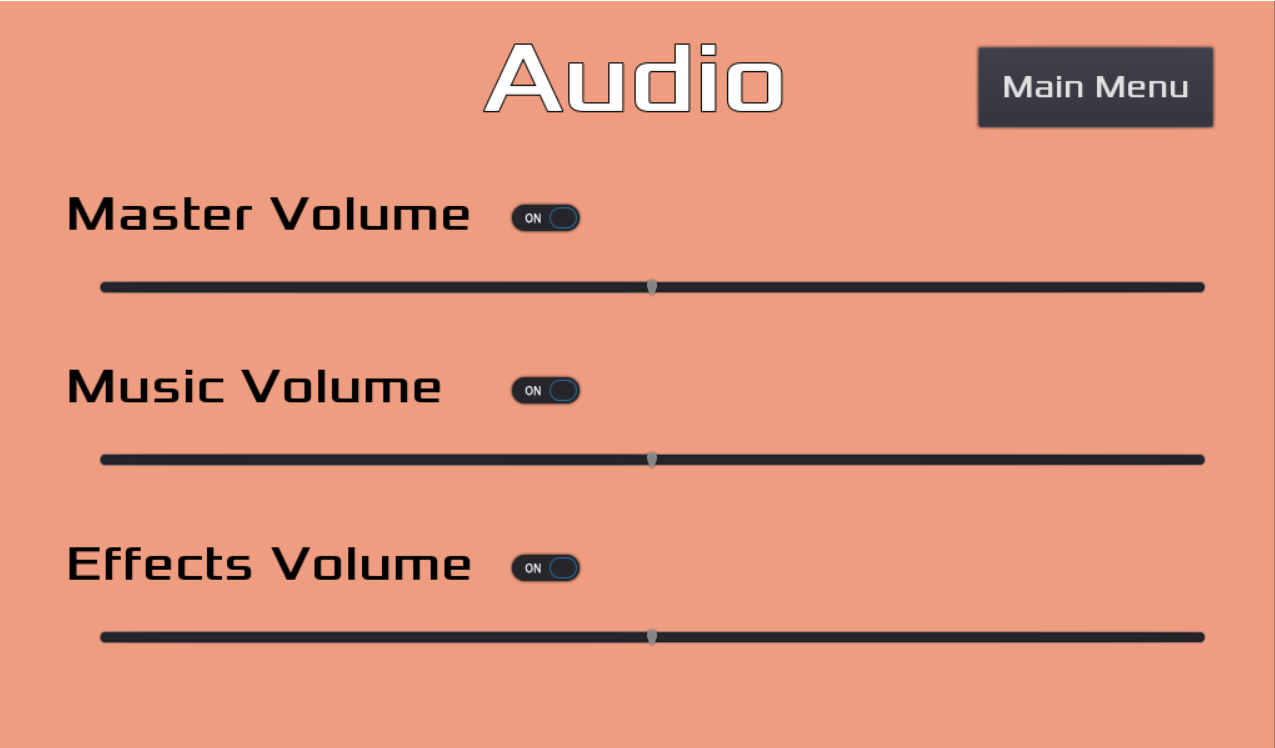
\includegraphics[width=0.8\linewidth]{figures/AudioMenu}
	\caption{Menú de configuración de sonido.}
	\label{fig:AudioMenu}
\end{figure}

\vspace{\baselineskip}

En el futuro, planeamos aumentar las opciones de configuración. Por un lado, habría que añadir una opción para configurar los controles y \emph{keybindings} (ej.: que se pueda lanzar una habilidad pulsando la tecla 1 en vez de Q). Por otro lado, habría que añadir un menú para configurar el apartado gráfico, para así permitir que aquellos jugadores con un PC de gama baja puedan jugar al juego con una buena tasa de FPS.

% ==============================================================================

\subsection{Modos de juego}
% \textit{Detallar los modos de juego que el usuario tendrá disponible. Para cada modo de juego, proporcionar una descripción detallada y si inicialmente es un modo que está bloqueado, incluir instrucciones para que el usuario sepa como tiene que desbloquearlo.}

Inicialmente se proponen los siguientes modos de juego, disponibles desde el primer momento (aunque el jugador no puede elegir cuál va a jugar en la próxima partida):
\begin{enumerate}
	\item \textbf{Deathmatch}: Modo 2vs2 en el que, para ganar, los jugadores de un equipo deberán matar 5 veces a los jugadores del otro equipo (puede ser 5 veces al mismo jugador o estar repartidas las muertes entre los dos jugadores enemigos). Cuando un jugador muere, \emph{respawnea}.
	
	\item \textbf{Captura}: Modo 2vs2 donde los jugadores deben defender una zona alrededor de un hada que se va moviendo por todo el mapa. Los equipos reciben puntos por cada jugador que esté dentro de la zona del hada en cada instante de tiempo. Una vez que han pasado 5 minutos, el equipo con más puntos gana. Cuando un jugador muere, \emph{respawnea}.
	
\end{enumerate}

\subsection{Arquitectura multijugador}
Para reducir al mínimo la latencia y simplificar el networking, se seguirá una esquema cliente-servidor, con servidor autoritario. Es importante evitar el envío de información redundante notificando únicamente de los cambios en el juego, es decir, el uso de actualizaciones en modo delta.

\vspace{\baselineskip}

La arquitectura se forma por un servidor autoritario, el cúal tienen su propia versión del juego, y se encarga de llevar la lógica. Cada jugador tiene la versión del cliente, la cuál durante la partida solo es responsable de actualizar la pantalla según los cambios indicados por el servidor y transmitir los comandos (ratón/teclado) introducidos por el usuario hacia este.
El servidor cuenta con una interfaz visual simple, permitiendo ver el estado de la partida con una representación gráfica simplificada.

El intercambio de mensajes se realizará usando la capa de networking que proporciona Godot, usando RTC con variantes TCP y UDP. El intercambio de mensajes continuos (donde se permite la pérdida de mensajes), como la posición de un personaje, se realizará mediante el protocolo UPD, y aquellos mensajes de gran importancia, como la notificación de crear un proyectil, harán uso de TCP.

Para no sobrecargar al servidor con entradas del usuario no válidas, el cliente también adicionalmente comprobará el estado de los cooldown antes de realizar las peticiones (pero manteniendo la responsabilidad de estos en el servidor para que no exista desfase entre ellos).

\vspace{\baselineskip}

Para un estado más avanzado del juego, sería recomendable fijar los envíos de mensajes en intervalos de tiempo concretos, reduciendo la latencia y estructurando el envío de mensajes. Esta técnica es usada en otros juegos del género asegurando la emisión de los paquetes a intervalos de frames regulares.